\section{I Thread}
Ci sono alcune applicazioni che richiedono la gestione in parallelo, ovvero quando viene programmata un'applicazione
viene suddivisa in piú parti, quindi l'applicazione rimane un singolo processo, ma che al suo interno esegue
piú computazioni in parallelo, quindi possiamo dire che un processo puó essere composto da piú thread.
In questo caso é compito del programmatore occuparsi della sincronizzazione tra i thread, il sistema operativo
si occupa di gestire i processi, mentre il programmatore si occupa di gestire i thread.
Diversi thread condividono molte risorse, del processo, non condividono lo stack delle chiamate ed anche il processore,
condividono invece memoria(Stack Esclusi), files, dispositivi di I/O, ecc.
Teoricamente si puó dire che il processo incorpori gestione delle risorse e scheduling
\begin{figure}[H]
    \centering
    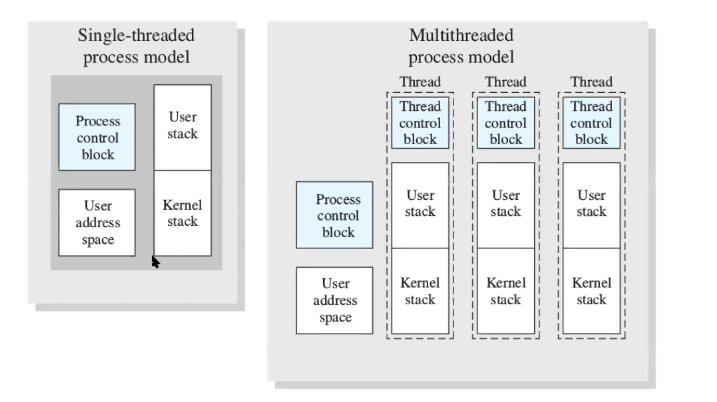
\includegraphics[width=0.5\textwidth]{immagini/thread1}
    \caption{Thread}
\end{figure}
Se sono su un sistema operativo Single Threaded, il sistema operativo non supporta il multithreading, ho l'immagine del processo
ed il PCB, se il sistema operativo supporta il multithreading, ho l'immagine del processo, il PCB e il TCB(Thread Control Block),
dove Il TCB gestisce solo la parte dello scheduling
\subsection{Perché introdurre i thread}
Creare un thread é semplice/efficiente, la creazione la terminazione, fare lo switching e farli comunicare,
quindi ogni processo viene creato con un thread, dopo il programmatore puo' creare altri thread con il comando spawn()
, esistono chiamate di sistema per bloccare un thread, sbloccare un thread, terminare un thread.
\subsection{ULT e KLT}
Esistono 2 tipi di thread:
\begin{itemize}
    \item ULT(User Level Thread): A livello di sistema operativo i thread non esistono, oppurtune librerie si occupano di gestire il thread
    \item KLT(Kernel Level Thread): Il sistema operativo supporta i thread, quindi il sistema operativo é a conoscenza dei thread
    \item
\end{itemize}
\begin{figure}[H]
    \centering
    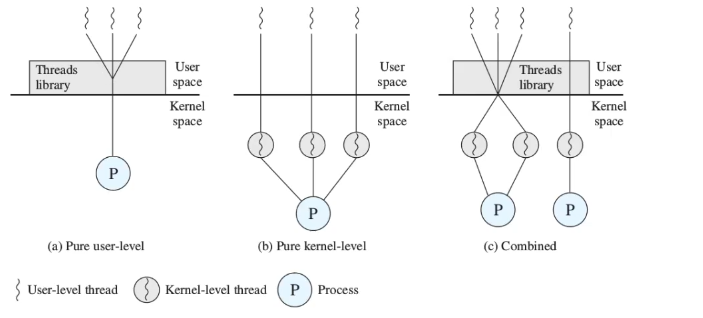
\includegraphics[width=0.5\textwidth]{immagini/ULTeKLT}
    \caption{ULT e KLT}
\end{figure}
perché usare ULT:
\begin{itemize}
    \item Sono piú veloci da creare e gestire (Non serve fare il mode swithcing)
    \item Si puó avere una politica di scheduling per ogni processo
    \item Permettono di usare i thread anche sui sistemi operativi che non li offrono nativamente
\end{itemize}
perché NON usare ULT:
\begin{itemize}
    \item Se un thread si deve bloccare, si bloccano tuitti i thread del processo, a meno che il blocco non sia chiamato
    dalla chiamata di block, al contrario con i KLT solo il thread che si blocca viene bloccato
    \item Se ci sono piú processori o piú core, i thread non possono essere eseguiti in parallelo perché il sistema operativo
    non é a conoscenza dei thread
\end{itemize}
\subsection{Processi e Thread in Linux}

I thread sono spesso associati al termine Light Weight Processes o LWP. Questo termine risale ai tempi in cui Linux supportava i thread solo a livello utente. Ciò significa che anche un'applicazione multithread era vista dal kernel come un singolo processo. Questo creava grandi sfide per la libreria che gestiva questi thread a livello utente, poiché doveva garantire che l'esecuzione di un thread non fosse ostacolata se un altro thread emetteva una chiamata bloccante.

Successivamente l'implementazione è cambiata, e ai processi sono stati collegati singoli thread, in modo che fosse il kernel a gestirli. Tuttavia, come discusso in precedenza, il kernel Linux non li vede come thread: ogni thread è trattato come un processo all'interno del kernel. Questi processi sono conosciuti come processi leggeri o light weight processes.

La principale differenza tra un processo leggero (LWP) e un processo normale è che gli LWP condividono lo stesso spazio di indirizzamento e altre risorse come i file aperti. Poiché alcune risorse sono condivise, questi processi vengono considerati più "leggeri" rispetto agli altri processi normali, da cui il nome di processi leggeri.

Quindi, in sostanza, possiamo dire che thread e processi leggeri sono la stessa cosa. È solo che thread è un termine usato a livello utente, mentre light weight process è un termine utilizzato a livello di kernel.


Nel kernel, ogni thread ha il proprio ID, chiamato PID (anche se forse avrebbe più senso chiamarlo TID), e ha anche un TGID (Thread Group ID) che corrisponde al PID del thread che ha avviato l'intero processo.

Semplificando, quando viene creato un nuovo processo, appare come un thread in cui sia il PID che il TGID sono lo stesso nuovo numero.

Quando un thread avvia un altro thread, il thread avviato ottiene il proprio PID (in modo che lo scheduler possa programmarlo indipendentemente), ma eredita il TGID dal thread che lo ha creato.

In questo modo, il kernel può programmare i thread indipendentemente dal processo a cui appartengono, mentre i processi (gli ID del gruppo di thread, o TGID) vengono mostrati agli utenti.

Per ogni thread, esiste quindi un PCB per ogni thread, questo crea un piccolo overhead perché esiste una duplicazione di alcune informazioni(puntatori)
\subsection{Gli stati dei processi in Linux}
Linux ha 5 stati per i processi, linux non distingue tra ready e running, divide peró in due stati blocked,
\begin{itemize}
    \item Task Running: il processo é in esecuzione sulla CPU
    \item Blocked:
    \begin{enumerate}
        \item Task Interruptible: il processo é in attesa di un evento, ma puó essere interrotto
        \item Task Uninterruptible: il processo é in attesa di un evento, ma non puó essere interrotto
        \item Task Stopped: il processo é stato fermato
        \item Task Traced: il processo é tracciato
    \end{enumerate}
    \item EXIT Zombie: il processo é terminato, ma il processo padre non ha ancora comunicato al sistema operativo
    \end{itemize}
\subsection{Segnali ed interrupt in Linux}
Non bisogna confondere i segnali con gli interrupt, I segnali possono essere inviati da un processo ad un altro processo,
quello che succede che il campo del PCB viene aggiornato con il segnale che é stato inviato, quando il processo
viene schedulato, il kernel controlla se ci sono segnali da gestire se si esegue la funzione di gestione del segnale,
alcuni signa handlers possono essere sovrascritti dal programmatore, alcuni segnali hanno l'handler non sovrascrivibile,
in ogni caso sono eseguiti in user mode, mentre gli interrupt sono eseguiti in kernel mode.
    